\item Three identical discs \(A\), \(B\), and \(C\) (Fig. 1.45) rest on a smooth horizontal plane. The disc \(A\) is set in motion with velocity \(v\) after which it experiences an elastic collision simultaneously with the discs \(B\) and \(C\). The distance between the centres of the latter discs prior to the collision is \(\eta\) times greater than the diameter of each disc. Find the velocity of the disc \(A\) after the collision. At what value of \(\eta\) will the disc \(A\) recoil after the collision; stop; move on?
    \begin{center}
        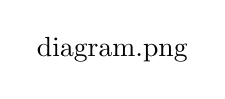
\begin{tikzpicture}
            \node at (0,0) {{diagram.png}};
        \end{tikzpicture}
    \end{center}
   
\begin{solution}
    \begin{center}
        \begin{tikzpicture}
            \pic at (0, 0) {frame=3cm};
        \end{tikzpicture}
    \end{center}
    
    \begin{align*}
        \intertext{From the symmetry of the problem, the velocity of the disk $A$ will be directed either in the initial direction or opposite to it just after the impact. Let the velocity of the disk $A$ after the collision be $v'$ and be directed towards right after the collision. It is also clear from the symmetry of the problem that the disks $B$ and $C$ have equal speed (say $v''$) in the directions shown. From the condition of the problem,}
        \cos\theta &= \dfrac{\eta}{d} = \dfrac{\eta}{2} \quad \text{so,} \quad \sin\theta = \sqrt{4-\eta^2}/2 \tag{1}
        \intertext{For the three disk system, from the conservation of linear momentum in the symmetry direction (towards right)}
        mv &= 2mv''\sin\theta + mv'' \quad \text{or} \quad v = 2v''\sin\theta + v'' \tag{2}
        \intertext{From the definition of the coefficient of restitution, we have for disks $A$, $B$ and $C$}
        e &= \dfrac{v''-v'\sin\theta}{v \sin\theta - 0}
        \intertext{But $e = 1$, for perfectly elastic collision.}
        v \sin\theta &= v'' - v'\sin\theta \tag{3}
        \intertext{From Eqs.~(2) and (3)}
        v' &= \dfrac{v(1-2\sin^2\theta)}{(1+2\sin^2\theta)} \\
        &= \dfrac{v(\eta^2-2)}{6-\eta^2} \quad \text{(using Eq.~1)}
        \intertext{Hence, we have,}
        v' &= \dfrac{v(\eta^2-2)}{6-\eta^2}
        \intertext{Therefore, the disk $A$ will recoil if $\eta < \sqrt{2}$ and stop if $\eta = \sqrt{2}$.}
        \intertext{Note: One can write the equations of momentum conservation along the direction perpendicular to the initial direction of disk $A$ and the conservation of kinetic energy instead of the equation of restitution.}
    \end{align*}
\end{solution}
